
\chapter{OpenFOAM}
\lhead{OpenFOAM}
\begin{refsection}
\chapterauthor{Gregor Dengler}
\section{Einleitung}
\rhead{Einleitung}
\index{OpenFOAM}
OpenFOAM (Open Source Field Operation and Manipulation) ist ein in
C++ geschriebenes, numerisches, freies Simulationssoftwarepaket. Es
wurde urspr"unglich in den sp"aten 1980er Jahren am Imperial College
in London entwickelt. OpenFOAM war jedoch nicht von Anfang an Open
Source, erst im Jahr 2004 nachdem es verkauft wurde, wurde es als
OpenFOAM ver"offentlicht. Das Ziel war ein Softwarepaket zu erstellen,
welches flexibler und besser als das bis dato genutze FORTRAN (Formula
Translating System) ist.
\index{FORTRAN}

OpenFOAM besteht nicht nur aus den Solvern f"ur die verschiedenen
Probleme, sondern besitzt auch Pre-Processing sowie Post-Processing
Tools. Im Pre-Processing wird vor allem ein Meshing Tool zur Verf"ugung
gestellt. Im Post-Processing wird mittels ParaView eine "ubersichtliche
Darstellung der berechneten Daten erm"oglicht. \cite{ofwiki}
\index{Pre-Processing}
\index{Post-Processing}

Im Pre-Processing wird die Geometrie definiert und Randbedingungen
vorgegeben. Es wird also definiert, was genau simuliert werden
soll. Randbedingungen sind Vorgaben zum Verhalten der Simulation am
Rande des simulierten Bereichs, sowie auf Oberfl"achen.

W"ahrend des solven, dem L"osen der Str"omungsdiffereitialgleichungen oder
\index{Solver}
allgemein der Feldgleichungen, wird die eigentliche Berechnung von Solver
ausgef"uhrt. Solver sind Programme, welche die Algorithmen von OpenFOAM
zur L"osung von partitiellen Differenzialgleichungen beinhalten.

Das Post-Processing soll die Berechnung visualisiert werden. Des Weiteren
k"onnen im Post-Processing auch physikalisch relevante Gr"ossen aus der
Berechnung extrahiert werden.
\begin{figure}
\begin{center}
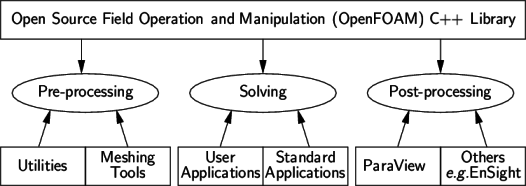
\includegraphics[width = 0.65 \linewidth]{./openfoam/pics/Aufbau.png}
\end{center}
\caption{OpenFOAM im "Uberblick \cite{of} }
\end{figure}

\section{Einsatzgebiete von OpenFOAM}
\rhead{Einsatzgebiete von OpenFOAM}
Es gibt in OpenFOAM eine ganze Reihe verschiedener Standard Solver f"ur diverse Probleme. Hier eine kleine "Ubersicht, f"ur welche Bereiche es bereits Standard Solver gibt:
\setlist{nolistsep}
\begin{itemize}
\setlength{\itemsep}{2pt}
\setlength{\parsep}{2pt}
\item Basic CFD codes  
\item Incompressible flow 
\begin{itemize}
\item \textbf{icoFoam}
\item \textbf{pisoFoam}
\end{itemize}
\item Compressible flow 
\item Multiphase flow
\item Direct numerical simulation (DNS) and large eddy simulation (LES)
\item Combustion
\item Particle-tracking flows
\item Heat transfer and buoyancy-driven flows
\item Molecular dynamics methods
\item Direct simulation Monte Carlo methods
\item Electromagnetics
\item Stress analysis of solids
\item Finance
\end{itemize} 

Da OpenFOAM Open Source ist und zudem sehr flexibel, wird es h"aufig in
der Forschung eingesetzt. Der Vorteil liegt darin, dass nicht nur der
Solver an sich, sondern auch die konkrete nummerischen L"osungsverfahren
f"ur die verschiedenen Gleichungen leicht eingestellt werden k"onnen. Man
hat zudem die M"oglichkeit, sich nebst den Standard Solvern auch Eigene
zu erstellen. So l"asst sich OpenFOAM mit einem gewissen Aufwand auf
jedes Problem zuschneiden. \cite{of}

\section{Beispiel Cavity}
\rhead{Beispiel Cavity}
\subsection{Pre-Processing}
\index{Cavity}
\begin{figure}
\begin{center}
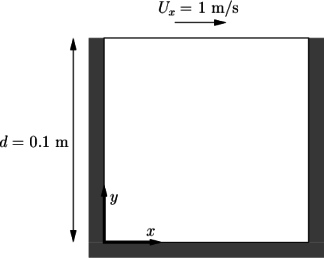
\includegraphics[width =  0.5\linewidth]{./openfoam/pics/cavity1.png} 
\end{center}
\caption{Beispiel Cavity \cite{of}\label{of:cavity}}
\end{figure} 
Ich habe mit dem Tutorial Beispiel Cavity und dem Solver IcoFOAM
begonnen. Im Beispiel Cavity geht es um die Simulation einer Str"omung,
die entsteht, wenn oberhalb einer offenen Box ein Luftzug durchweht
(Abbildung\ref{of:cavity}). Es
interessiert also in diesem Beispiel lediglich, was innerhalb der Box
geschieht. Grunds"atzlich muss beim Beispiel Cavity nichts mehr gemacht
werden, es ist bereits alles voreingestellt. Man sieht gut wie ein
OpenFOAM Projekt aufgebaut sein sollte. Zudem l"asst sich der Einfluss
der Anzahl Zellen und der Simulationszeit einfach veranschaulichen.


\begin{figure}
\begin{center}
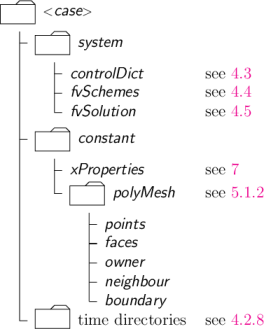
\includegraphics[width =  0.4\hsize]{./openfoam/pics/Struktur.png}
\end{center}
\caption{Ordnerstrucktur eines OpenFOAM Projekts \cite{of}\label{of:struktur}}
\end{figure}
Im Bild~\ref{of:struktur} sieht man die Ordnerstruktur eines OpenFOAM Projekts.
In den verschiedenen Files lassen sich verschiedene Parameter einstellen.

Im Ordner  \texttt{system} ist alles grunds"atzliche definiert. So wird
im File  \texttt{controlDict} festgelegt, welcher Solver verwendet
werden soll, hier z.B. icoFOAM. Dann wird der Start sowie das Ende
der Simulation definiert. In diesem Beispiel wird eine Startzeit von
0 s festgelegt und eine Endzeit von 0.5s. Des Weiteren werden die
Zeitschritte festgelegt, hier 0.005s. Es werden noch weitere Parameter
eingestellt, wie Ausgabeformat usw.

Im File  \texttt{fvSchemes} wird vorgegeben, welche nummerischen
L"osungsverfahren zur L"osung der Gleichungen verwendet werden sollen.

Im File \texttt{fvSolution} wird f"ur jede Art Gleichung eine
L"osungsalgorithmus bestimmt.  Hier stehen Algorithmen zur Auswahl,
die in fr"uheren Kapiteln dieses Buchs erl"autert wurden. So z.B. Der
Gauss-Seidel Algorithmus.



Im Ordner  \texttt{constant} wird vor allem die Form des zu simulierenden
Gegenstands bestimmt. Das Ganze geschieht mit dem Tool blockMesh. Um
es zu nutzen, muss zuerst in einem Text-File jeder Punkt der ben"otigt
wird mit seinen $x$-$y$-$z$ Koordinaten bestimmt werden. In diesem Fall muss
nur ein Block erstellt werden, d. h. insgesamt 8 Punkte.

\definecolor{ofback}{RGB}{240,240,240}
\lstnewenvironment{ofcode}[1][]
  {\lstset{
        backgroundcolor =               \color{ofback},
    language =                          C++,
    basicstyle =                	\ttfamily,
    breaklines =                        true,
    frame =                             none,
    columns =                           flexible,
    keepspaces =                        true,
    showstringspaces =          	false,
    extendedchars =                     true,
    numbers =                           left,
    numbersep =                         2pt,
    numberstyle =                       \tiny,
    rulecolor =				\color{black},
    stepnumber =                        1,
    tabsize =                           8,
  }}{\vspace{0em}}
\lstset{
        backgroundcolor =               \color{ofback},
    language =                          C++,
    basicstyle =                	\ttfamily,
    breaklines =                        true,
    frame =                             none,
    columns =                           flexible,
    keepspaces =                        true,
    showstringspaces =          	false,
    extendedchars =                     true,
    numbers =                           left,
    numbersep =                         2pt,
    numberstyle =                       \tiny,
    rulecolor =				\color{black},
    stepnumber =                        1,
    tabsize =                           8,
}

Nachstehend sieht man Ausz"uge aus dem File \texttt{blockMeshDict}. Unter
\texttt{vertices} sind die erw"ahnten 8 Punkte definiert.  Da man hier
eine eigentlich 2 dimensionale Simulation machen will und Effekte der
dritten Dimension nicht interessieren, sind die Punkte in der dritten
Dimension sehr nahe bei einander. OpenFOAM kann keine 2D Simulationen,
also muss man sich hier selbst etwas zu helfen wissen.
\begin{ofcode}
convertToMeters 0.1;
vertices
(
	(0 0 0)
	(1 0 0)
	(1 1 0)
	(0 1 0)
	(0 0 0.1)
	(1 0 0.1)
	(1 1 0.1)
	(0 1 0.1)
);
\end{ofcode}

Im folgenden Codeblock sieht man, wie so ein Block
definiert wird. In der ersten Klammer sind die Punkte, welche den Block
begrenzen. Hier ist es wichtig die Reihenfolge der Punkte zu beachten. Die
Zahl entspricht der unter \texttt{vertices} genanten Punkte in der
Reihenfolge, in der sie genant werden.
\begin{ofcode}
blocks
(
	hex (0 1 2 3 4 5 6 7) (20 20 1) simpleGrading (1 1 1)
);
\end{ofcode}

Definiert man seine Blocks in der falschen Reihenfolge, so ver"andert man
die Form der Blocks. Da \texttt{blockMesh} die Linie, welche den Block
begrenzt genau der Reihenfolge nach zieht, in der die Punkte in der
Klammer genannt werden. In der zweiten Klammer defniert man, wieviele
Zellen in welcher Dimension angelegt werden sollen.  Hier sind das 20
in X sowie Y Richtung und 1 in Z Richtung. Dies weil es eigentlich eine
2D Simulation werden soll.

Das n"achste Codefragment zeigt, wie die verschiedenen \texttt{Walls}
definiert werden. Auch hier sind in den Klammern die Punkte, welche die
Wall definieren aus\texttt{vertices} genannt. In dieser Simulation gibt
es 3 Typen von Walls, die \texttt{movingWalls}, die \texttt{fixedWalls}
und  \texttt{frontAndBack}. Unter \texttt{movingWalls} ist die
Wand, welche f"ur uns am interessantesten ist, da sie den offenen
Teil der Box darstellt. Hier soll die Str"omung durchfliessen. Die
\texttt{fixedWalls} sind die W"ande der Box, die simuliert werden
soll. Unter \texttt{frontAndBack} sind die beiden Walls gemeint, welche
die Front- und R"uckansicht darstellen und auf diese Simulation keinen
Einfluss haben sollen. Deshalb sind diese Walls als \texttt{empty}
definiert.
\begin{ofcode}
boundary
(
	movingWall
	{
		type wall;
		faces
		(
			(3 7 6 2)
		);
	}
	fixedWalls
	{
		type wall;
		faces
		(
			(0 4 7 3)
			(2 6 5 1)
			(1 5 4 0)
		)
	}
	frontAndBack
	{
		type empty;
		faces
		(
			(0 3 2 1)
			(4 5 6 7)
		)
	}
);
\end{ofcode}

\texttt{Time directories} ist ein "Uberbegriff f"ur eine ganze Reihe von
Ordnern. Wenn man keine Ver"anderungen der grunds"atzlichen Situation
w"ahrend der zu simulierenden Zeit machen will, muss man lediglich einen
Ordner  \texttt{0} erstellen. In diesem Ordner wird alles definiert,
was w"ahrend der Simulation nicht "andert. Im Beispiel Cavity sind die
Variablen  \texttt{p} und  \texttt{U} vordefiniert.
Im File \texttt{p} wird der
Anfangsdruck und im File \texttt{U} die Anfangsgeschwindigkeit bestimmt.
Wenn man
nun noch eine Ver"anderung w"ahrend der Simulation erreichen will, so
m"usste man das entsprechende Verzeichnis erstellen und die Ver"anderung
darin definieren.

\subsection{Berechnung}
Sind nun alle Voreinstellungen gemacht, l"asst sich die Berechnung
mittels Befehl \texttt{icoFOAM} starten. Alternativ kann man mit OpenMPI auch
eine parallele Berechnung auf mehreren Prozessoren durchf"uhren. Daf"ur
wird eine kleine Vorbereitung ben"otigt. Es muss in einem weiteren
Textfile namens \texttt{decomposeParDict} definiert werden, auf wie
viele Prozessoren die Arbeit verteilt werden soll. Des Weiteren muss
man definieren wie die Arbeit aufgeteilt wird. So kann man angeben, wie
viele Unterteilungen es in jeder Dimension geben soll. Ein weiter Punkt,
der definiert wird, ist die, wie sehr der Rechenaufwand pro Prozessor
voneinander abweichen darf. Danach wird das \texttt{decomposePar}
gestartet und der Computer erstellt f"ur jeden Prozessor ein eigenes
Verzeichnis. Nun ist die Arbeit fertig aufgeteilt. Jetzt kann man
die Simulation starten. Das wird mit dem Befehl \texttt{mpirun -np 16
icoFoam -parallel} gemacht. Hier ist wichtig, dass der Funktion icoFoam
die Option parallel mit "ubergeben wird, da sonst trotz Vorbereitung
nur auf einem Prozessor gerechnet wird.

Ist die Berechnung abgeschlossen, muss man im Falle
der parallelen Berechnung die Daten der verschiedenen
Prozessoren wieder zusammenf"ugen. Dies geschieht mit dem Befehl
\texttt{reconstructPar}. Dieser Befehl macht aus den verschiedenen
Verzeichnissen der verschiedenen Prozessoren wieder ein Verzeichnis in
dem alle Ergebnisse sind. Erst dann lassen sie sich mittels ParaFOAM
visualisieren.

\subsection{Post-Processing}
Sind die Daten nach dem parallelen Berechnen wieder richtig
zusammengef"ugt, so lassen sich diese nun mit dem Befehl paraFoam
anschauen. Es wird nun paraView ge"offnet und man kann sich die
verschiedenen Daten anzeigen lassen.
\begin{figure}
\begin{center}
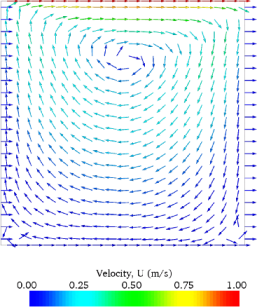
\includegraphics[width = 0.31\hsize]{./openfoam/pics/stroemung.png}
\qquad
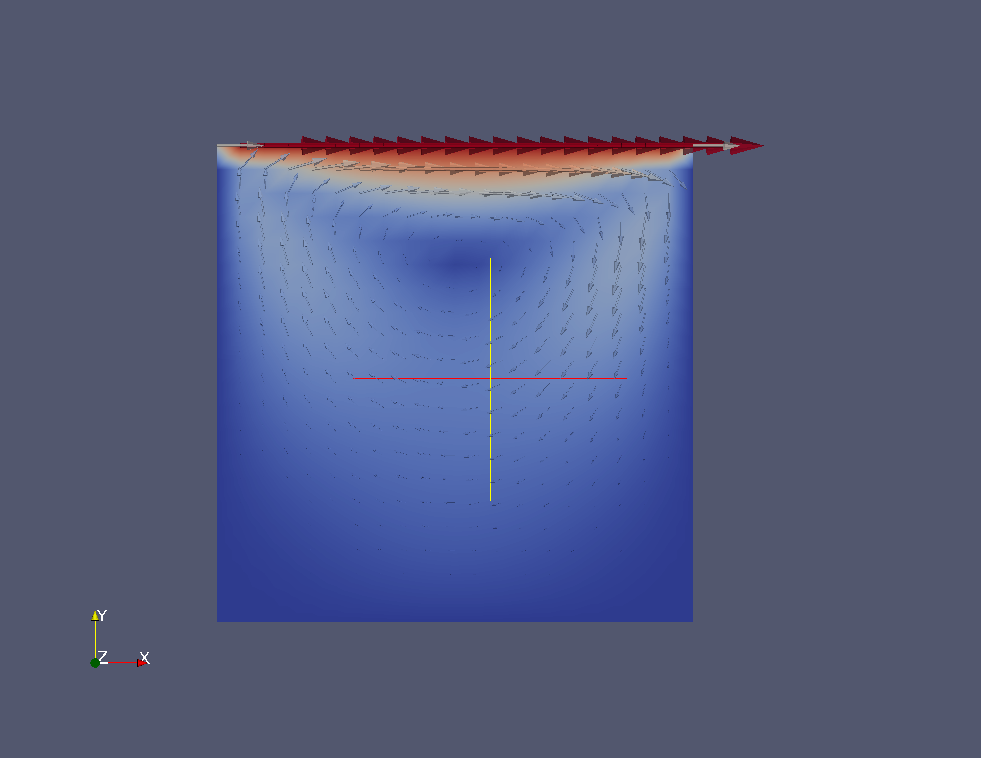
\includegraphics[width = 0.48\hsize]{./openfoam/pics/stroemung2.png}
\end{center}
\caption{Cavity Vektoransicht (links) und Str"omungsansicht (rechts)
\cite{of}}
\end{figure}

Auf diesen Bildern ist die Str"omung innerhalb der Box sehr gut zu
erkennen. Es bildet sich innerhalb der Box ein Wirbel, wie man das von
Anfang an erwartet hat. Es l"asst sich in ParaView aber nicht nur der
Schlusszeitpunkt anschauen. Man kann auch den Verlauf der Str"omung in
einer Art Video ansehen.

\section{Beispiel Keil}
\rhead{Beispiel Keil}
\index{Keil}
Das Beispiel Keil habe ich selber versucht mit Cavity als Grundlage zu
erarbeiten. Im Grundsatz geht es um einen Keil, der in einem Windkanal
in einer Str"omung steht. In diesem Beispiel erwarte ich, dass sich
hinter dem Keil ein gr"osserer Wirbel bilden wird. Um nun in diesem
intressanten Bereich genug Daten zu sammeln empfiehlt es sich, in diesem
Bereich etwas mehr Zellen zu generieren. Daf"ur muss der Raum hinter
dem Keil in mehrere Bl"ocke eingeteilt werden.

\subsection{Mesh}
In diesem Beispiel hab ich, nach anfangs gescheitertem Versuch mit gmsh,
mit dem blockMesh von OpenFoam gearbeitet. Wie schon erw"ahnt, habe ich
hierf"ur alle Punkte von Hand in ein Textfile geschrieben. In diesem
Beispiel bedeutet das 174 Punkte. Zus"atzlich muss man noch alle Bl"ocke
als solche definieren, hier 23. Als Letztes werden alle Aussenfl"achen
definiert, hier waren das 65 Fl"achen.

Mit den hier definierten Blocks unterteilt man die Berechnung. Man
kann so an interessanten Stellen mehr Zellen erzeugen und an weniger
interessanten Stellen weniger. Sind 2 Bl"ocke direkt benachbart, so
erkennt das OpenFOAM. Hierf"ur ist es aber notwendig, dass die Punkte
in richtiger Reihenfolge eingegeben wurden. F"ur alle Blocke die am
Rand sind, muss f"ur die aussenliegenden Fl"achen definiert werden, was
sie f"ur einen Einfluss auf die Simulation haben. In dieser Simulation
sind das alle Fl"achen oben und unten sowie an den Seiten des Windkanals
die keinen Einfluss haben sollen und die Fl"ache vorne und hinten welch
offen sein sollen. Die Fl"achen des Keils selber sollen sich wie fixe
W"ande verhalten.
\begin{figure}
\begin{center}
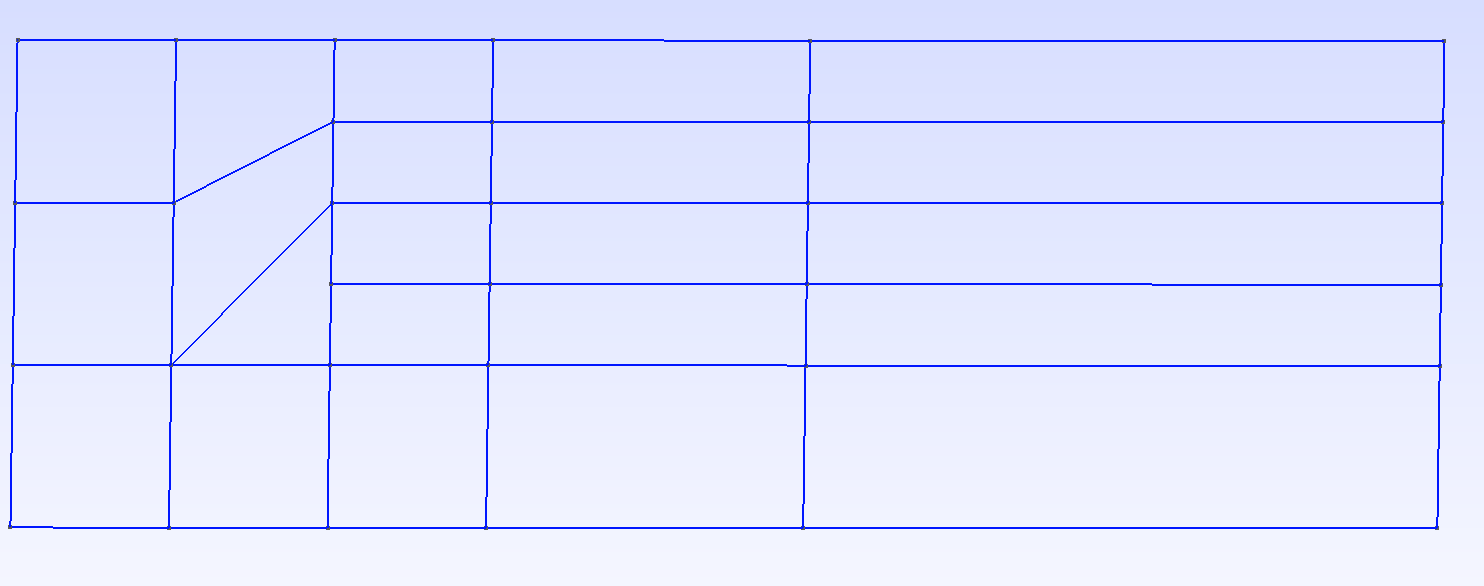
\includegraphics[scale = 0.2]{./openfoam/pics/Keil.png}
\end{center}
\caption{Mesh mit gmsh}
\end{figure}

Wie gut zu erkennen ist, ist der Keil ganz am Anfang des Windkanals. Das,
weil die interessanten Wirbel vor allem nach dem Keil entstehen werden
und man so genug davon sehen kann. Auch gut zu erkennen ist, dass ich die
Bl"ocke in unmittelbarer N"ahe zum Keil sehr klein gew"ahlt habe. Dies hab
ich so gew"ahlt, weil ich in jedem Block gleich viele Zellen definiert
habe. Man hat also rund um den Keil viel mehr und viel kleinere Zellen
als gegen Schluss des Windkanals. Ich habe in diesem Beispiel 200 x 200
Zellen pro Block gew"ahlt, also 23 x 200 x 200 (=920'00)Zellen.

\subsection{Die Courant-Zahl}
\index{Courant-Zahl}
Will man mit einer CFD (Computational Fluid Dynamics) Software etwas
\index{CFD}
berechnen, so hat man bei den Einstellungen zu beachten, dass die
Berechnung stabil bleibt. Um dies zu erreichen, muss die sogenannte
Courant-Zahl (auch Courant-Friedrichs-Lewy-Zahl genannt) zwingend unter
1 bleiben.
\[
c = \frac{u \cdot \Delta t}{\Delta x} < 1
\]

In meiner Simulation ist die h"ochste auftretende Geschwindigkeit $u$
die Schallgeschwindigkeit. Die gr"osste Ortschritt $\Delta x$ wird
durch die Zellengr"osse definiert. Will man eine erfolgreiche Simulation
durchf"uhren, muss man den Zeitschritt klein genug w"ahlen. Das Problem
mit kleinen Zeitschritten ist, dass man sehr viel Rechenaufwand hat,
w"ahlt man ihn aber zu gross so bricht die Simulation eventuell nach
einiger Zeit ab.

Bei der Simulation vom Keil wurde ein Zeitschritt von 0.1 ms gew"ahlt
um diese Bedingung zu erf"ullen.

\subsection{Berechnung}
Die Berechnung vom Beispiel Keil wurde auf 32 Cores gestartet. Insgesamt
wurde w"ahrend ca 6 Tagen auf allen 32 Cores mit Vollast gerechnet. In
dieser Zeit konnten 0.67 s der Simulation berechnet werden. Dass
entspricht ca 6,2 Mia. Berechnungen. In dieser Zeit wurden 8,7 GB Daten
generiert. Wie schon die etwas ungew"ohnliche Simulationszeit erahnen
l"asst, war urspr"unglich nicht geplant, nur 0.67 s zu simulieren. Es ist
jedoch nach 0.67 s zu einem "Uberschreiten der Courant-Zahl und somit
zum Abbruch wegen Divergenz gekommen. Dies, weil die Druck"anderung an
der Anfangspitze des Keil zu gross wurde und sie somit die Zellengr"osse
"ubersprang.

\subsection{Ergebnis}
Das Ergebnis l"asst sich mittels ParaView visualisieren. Man merkt beim
Begutachten der Resultate mit ParaView schnell, dass es sich um sehr
viele Daten handelt, da es sehr langsam l"auft. Das Ergebnis ist aber
so herausgekommen wie im Voraus erwartet. Es l"ost sich, wie anfangs
angenommen, an der oberen Spitze des Keils ein Wirbel ab. Was etwas
extremer ausf"allt als erwartet, ist die Kompression am Anfang des
Keils. An dieser Stelle entsteht ein sehr hoher Druck, was auch zum
Abbruch der Simulation gef"uhrt hat.
\begin{figure}
\begin{center}
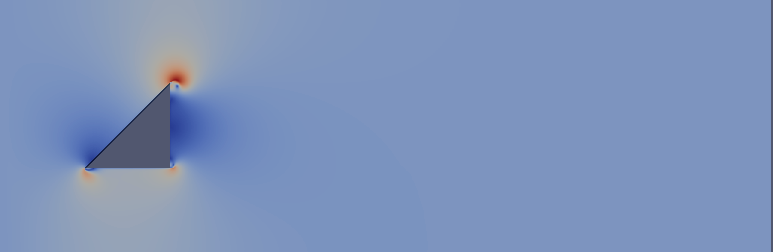
\includegraphics[width = 0.49\hsize]{./openfoam/pics/U1.png}
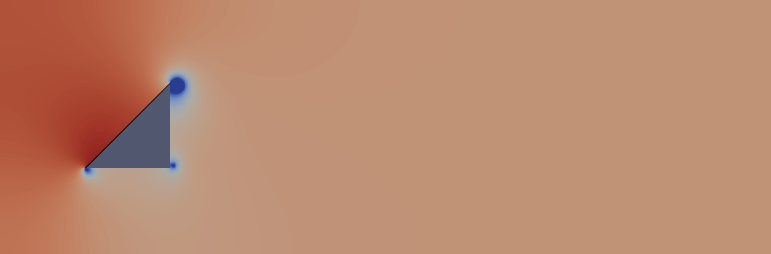
\includegraphics[width = 0.49\hsize]{./openfoam/pics/p1.png}
\\[0.5mm]
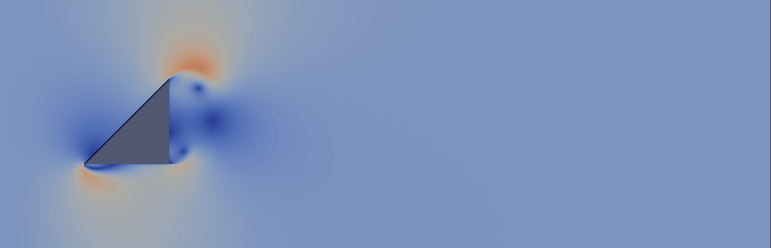
\includegraphics[width = 0.49\hsize]{./openfoam/pics/U5.png}
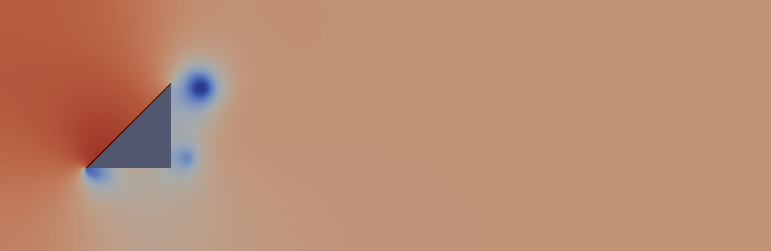
\includegraphics[width = 0.49\hsize]{./openfoam/pics/p5.png}
\\[0.5mm]
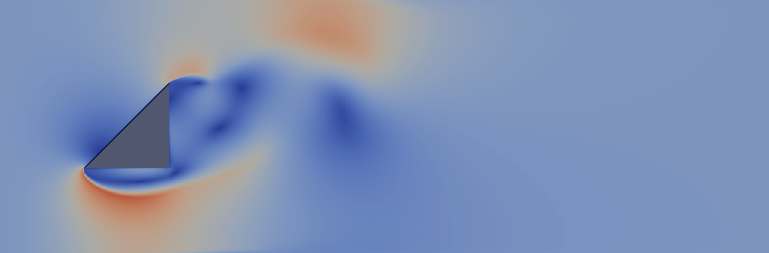
\includegraphics[width = 0.49\hsize]{./openfoam/pics/U25.png}
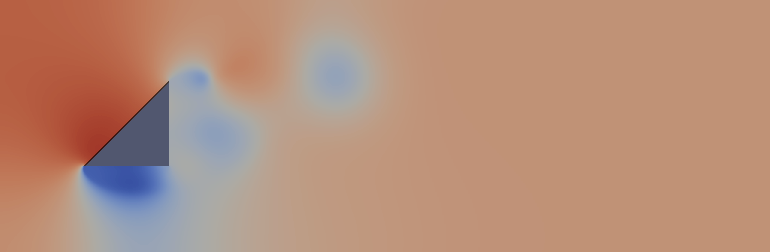
\includegraphics[width = 0.49\hsize]{./openfoam/pics/p25.png}
\\[0.5mm]
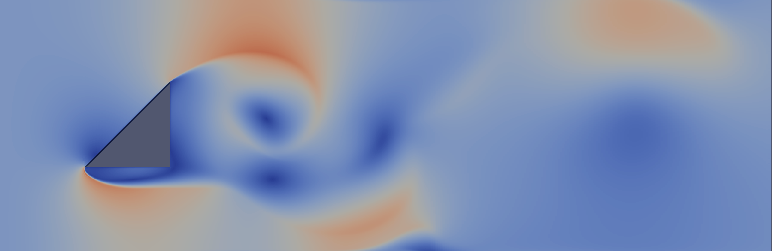
\includegraphics[width = 0.49\hsize]{./openfoam/pics/U55.png}
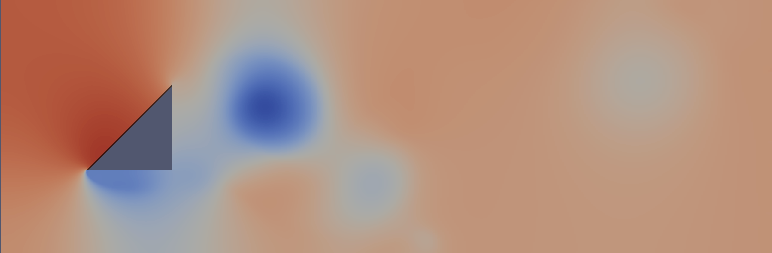
\includegraphics[width = 0.49\hsize]{./openfoam/pics/p55.png}
\end{center}
\caption{Bilder der Str"omungsgeschwindigkeit (links) und des Druckes
(rechts) nach 10, 50, 250, 550 ms}
\end{figure}

\section{Probleme}
\rhead{Probleme}
Ich hatte w"ahrend der Arbeit mit OpenFOAM mit Problemen zu k"ampfen. In
diesem Abschnitt wird beschrieben, wo ich am meisten Zeit verloren habe
und wie man sich diesen "Arger sparen kann.

\subsection{Installation}
W"ahrend meiner Arbeit mit OpenFOAM kostete alleine schon die Installation
sehr viel Zeit. Dies, weil ich den Fehler machte, eine nicht voll
kompatible OpenSuse Version zu verwenden. Das f"uhrte dazu, das ich das
vorbereitete Package nicht gebrauchen konnte und mir das Softwarepaket
aus dem Sourcecode selbst kompilieren musste.

Hierf"ur wurden diverse zus"atzlichen Packages ben"otigt, welche ich
selber korrekt installieren musste. F"ur mich als Linux-Anf"anger
war das nicht immer ganz einfach und ich musste mich oft auf Hilfe
von Mitbewohnern und Mitstudenten berufen. Schlussendlich brachte ich
das Softwarepaket fast zum Laufen. Das Einzige, was unter Linux nie
funktionierte, war die Visualisierung mit ParaView. Hier gab es ein
Problem mit der Software Paralles, welche die virtuelle Maschine, in
der Linux l"auft, betreibt.

Ich versuchte, das ganze unter Mac OS X zum Laufen zu bringen. Auch hier
mit bescheidenem Erfolg. Das einzige, was korrekt installiert wurde
unter Mac OS X war ParaView. Somit konnte ich die Berechnungen unter
Linux bzw. mittels HPC der HSR berechnen lassen und mit ParaView unter
Mac OS X visualisieren.

Beim n"achsten Mal w"urde ich nicht mehr versuchen, OpenFOAM in einer
virtuellen Maschine zu installieren, sondern auf einem Computer mit
nativ Linux. Dies h"atte mir viel Arbeit erspart.

\subsection{BlockMesh}
Mein zweites grosses Problem war, dass ich zwar versuchte, mit gmsh ein
Mesh meiner Simulation zu erstellen, dies aber am Einbinden ins OpenFOAM
scheiterte. Hier ist zu erw"ahnen, dass ich aufgrund der verlorenen
Zeit bei der Installation nicht alle M"oglichkeiten ausgesch"opft habe,
sondern ziemlich schnell entschied, mit BlockMesh und der Eingabe von
Hand ins Textfile mein Mesh zu erstellen.

Das Hauptproblem beim Blockmesh ist, dass man auch nach dem meshen
das Ergebnis nicht visualisieren kann, es ben"otigt also eine sehr
sorgf"altige Eingabe der verschiedenen Punkte und Blocks. Hier hatte
ich in einem meiner 174 Punkte in einer Dimension einen Tippfehler,
welchen ich selber nicht finden konnte. Herr M"uller entdeckte diesen
beim Untersuch meiner Probleme. \\ Danach konnte die Simulation, nach
Behebung weiterer kleiner Ungereimtheiten und nach fertigem Erstellen der
Files fvScheme und fvSolution, gestartet werden. Wie schon erw"ahnt brach
dann die Simulation nach 0.67 s Simulationszeit ab. Dies war aber nicht
weiter tragisch, da Herr M"uller am Abend, als es zum Abbruch kam, die
Simulation sowieso abbrechen wollte um die Ergebnisse f"ur die Vorlesung
Numb3rs @ HSR zu verwenden.

\section{Fazit}
\rhead{Fazit}
Mein pers"onliches Fazit zur Arbeit mit OpenFOAM f"allt nicht
besonders positiv aus, da es sehr aufw"andig ist, sich in OpenFOAM
einzuarbeiten. Ich bin mir aber sicher, dass wenn man das Softwarepaket
einmal im Griff hat, man seine Ziele auch innert n"utzlicher Frist
erreichen kann. Ich kann mir gut vorstellen, dass sich mit einigem
Training und gen"ugend einarbeiten in dieses Softwarepaket auch komplexe
Probleme l"osen lassen. Der grosse Vorteil von OpenFOAM gegen"uber den
kommerziellen L"osungen, wie z.B. COMSOL Multiphysics, welches z.B. im
Modul angewandter Elektromagnetismus Felder und Wellen eingesetzt wird,
ist, dass es Open Source ist und somit beliebig parallelisiert werden
kann, ohne f"ur jeden Thread eine Lizenz erwerben zu m"ussen. Kommerzielle
Softwarel"osungen, welche einen solch breiten Bereich abdecken, sind
in der Regel sehr teuer und somit l"asst sich mit OpenFOAM sehr viel
Geld einsparen. Ein weiterer Vorteil von Open Source Software ist,
dass man genau weiss, was und wie gerechnet wird. Es lassen sich auch
eigene Solver schreiben, wenn man z. B. ein Problem hat, f"ur das es
noch keinen gibt. Dies wiederum macht die Software sehr flexibel. Die
Tatsache, dass man jedes L"osungsverfahren selber definieren kann,
macht die Software noch flexibler. Hier kommt allerdings auch einer
der grossen Nachteile zum Tragen. Man muss genau wissen, was man macht,
da man sonst nicht auf ein gew"unschtes Resultat kommt.

Es gibt f"ur OpenFOAM sehr viele Forumbeitr"age, in denen diverse Probleme
gel"ost und erkl"art werden, jedoch ist es f"ur Anf"anger etwas schwierig,
da nicht alles sauber dokumentiert ist und man nicht immer versteht,
wie man gewisse Einstellungen richtig nutzt.
\printbibliography[heading=subbibliography]
\end{refsection}
